%!TEX root = ../main.tex

\section{Selection}
\label{sec:b02dd:selection}

The amount of background in \BdToDD is too high to perform a significant
measurement of \CP violation without any selection. The selection is divided
into three parts: a preselection with many high signal efficiency
requirements, a dedicated treatment of mis-identified backgrounds and a
multivariate analysis to further reduce combinatorial background.

\subsection{Preselection}
\label{sec:b02dd:selection:cuts}

Only events that have been triggered by a topological trigger line or by the
inclusive $\phi$ line and that in total contain less than \num{500} long
tracks are considered. All candidate kaon and pion tracks have to be long
tracks and have to satisfy quality criteria. Lower limits on the momentum ($p
> \SI{1}{\GeVc}$) and on the transverse momentum ($\pT > \SI{100}{\MeVc}$) are
required. The candidates should be inconsistent with originating from the PV
and the particle identification (PID) system needs to classify them as pions
or kaons with only a small probability to be a ghost.

Of all the possible combinations of three charged hadron tracks forming a
$\Dp$ meson candidate only the two possibilities \DToKpipi and \DToKKpi are
selected. The vertex needs to be significantly displaced from all PVs in the event
and the distance of the closest approach between all pairs of particles
forming the vertex has to be below \SI{0.5}{\mm}. The scalar sum of the \pT
has to exceed \SI{1800}{\MeVc} and the combined invariant mass has to be in
the range \SI{\pm25}{\MeVcc} around the nominal \Dp mass~\cite{PDG2014}. The
tightened mass window as well as requiring that the \chisq of the flight
distance of each $\Dpm$ meson with respect to the $\Bd$ decay vertex has to be
larger than \num{2} reduces the amount of (partially) charmless contributions.
On top of that, a cut on the decay time significance of the $\Dpm$ mesons,
defined as their decay time with respect to the $\Bz$ decay vertex divided by
the corresponding uncertainty, is supposed to further suppress the (partially)
charmless contributions. The optimal cut value is estimated under the
assumption that a very tight cut leaves only candidates with resonant $\Dpm$
mesons. Gradually loosening the cut the value can be found where the product
of the \Bd signal yield, extracted from a fit on data, and the signal
efficiency, determined on MC, exceeds the estimation from the initial tight
cut scenario. If both $\Dpm$ mesons are reconstructed via \DToKpipi decays the
decay time significance has to be greater than \num{0}. It needs to be greater
than \num{3} if one of the $\Dpm$ mesons is reconstructed in the \KKpi and the
other in the \Kpipi final state. Although in this case the final states
of the \Dpm mesons differ the same cut is applied to both \Dpm mesons as on
signal MC the comparison of the distributions of the decay time significance
shows a good agreement between \DToKpipi and \DToKKpi decays.

The vertex formed by a pair of oppositely charged $\Dpm$ candidates needs to
be of good quality. The scalar sum of the $\pT$ of the $\Dpm$ mesons must
exceed $\SI{5}{\GeVc}$. In the stripping a BDT to select $\Bd$ candidates is
applied. The BDT is based on the \pT and the flight distance \chisq of the \Bz
as well as on the sum of the \Bz and both \PD vertex \chisq's divided by the
sum of the degrees of freedom of these vertex fits. Moreover, the \Bd
candidates are required to have $p > \SI{10}{\GeVc}$ and to have
$\chisqip<\num{25}$, where $\chisqip$ is defined as the difference in the
vertex fit $\chi^2$ of the associated PV with and without the $B^0$ candidate.

The reconstructed decay time $t$ of the \Bd candidate is determined from a DTF
(see \cref{sec:dataanalysis:dtf}), in which the \Bd production vertex is
constrained to the position of the associated PV. Only candidates with decay
times in the range \SIrange{0.25}{10.25}{\ps} are kept. The invariant mass
$m_{\Dp\Dm}$ of the $\Bd$ candidate has to be in the range
\SIrange{5150}{5500}{\MeVcc}. It is calculated from a DTF, in which the
invariant masses of $\Kpipi$ and $\KKpi$ are additionally constrained to the
known $\Dp$ mass. It is required that these fits have converged. Further
outliers are removed by requiring that the uncertainty on the invariant mass
and on the decay time has to be below \SI{30}{\MeVcc} and \SI{0.2}{\ps},
respectively, and that the absolute value of the $z$ coordinate of the PV is
smaller than \SI{250}{\milli\meter}.

The signal efficiency of the preselection for the final state with two kaons
is $\SI{82}{\percent}$ at a background rejection of $\SI{94}{\percent}$. For
the final state with three kaons the signal efficiency is
$\SI{67.5}{\percent}$ at a background rejection of $\SI{98}{\percent}$.

\subsection{Vetoes}
\label{sec:b02dd:selection:vetoes}

A $K\rightarrow\pi$ mis-ID can lead to background contributions from
$\DspToKKpi$, which predominantly proceeds through $\DsTophipi$. To reduce
these $\Dsp$ contributions the kaon mass hypothesis is assigned to the pion
with the higher transverse momentum of $\DpToKpipi$ candidates. The candidate
is rejected if the invariant mass of the hypothetical kaon pair is compatible
with the $\phi$ mass of $M_{\phi} = \SI{1019.461}{\MeVcc}$~\cite{PDG2014}
within $\pm\SI{10}{\MeVcc}$ or if the invariant mass of the $\kaon\kaon\pion$
combination is compatible with the \Dsp mass of $M_{\Dsp} =
\SI{1968.30}{\MeVcc}$~\cite{PDG2014} within $\pm\SI{25}{\MeVcc}$ and the pion
with the higher \pT (the one that the kaon mass hypothesis is assigned to) has
a larger $\texttt{ProbNN}K$ than $\texttt{ProbNN}\pion$ probability. When
assigning the kaon mass hypothesis to the pion with the lower \pT no vetoes
are applied as no resonant structures at the $\phi$ or the $\Dsp$ mass are
found.

To reduce $p\rightarrow\pi$ mis-ID the proton mass hypothesis is assigned to
the pion with the higher \pT of $\DpToKpipi$ candidates. The candidate is
rejected if the invariant mass of the $\kaon\proton\pion$ combination is
compatible with the \Lc mass of $M_{\Lc} =
\SI{2286.46}{\MeVcc}$~\cite{PDG2014} within $\pm\SI{25}{\MeVcc}$ and the
proton probability $\texttt{ProbNN}p$ of the pion with the higher \pT is
larger than $\texttt{ProbNN}\pion$.

\subsection{Multivariate analysis}
\label{sec:b02dd:selection:mva}

\subsubsection*{BDT training}
\label{sec:b02dd:selection:mva:training}

To further suppress combinatorial background a Boosted Decision Tree
(BDT)~\cite{Breiman,Roe} based on the implementation in
TMVA~\cite{Hocker:2007ht} is trained using a signal MC sample and the upper
mass sideband with $m_{\Dp\Dm} > \SI{5500}{\MeVcc}$. The training is performed
on half of these samples while the other half is used to test the BDT
performance. The selection steps described above, are applied before the
training.

Two BDTs separated by the number of kaons in the \Bd final state are trained.
The importance of the \num{21} features of the training differs, which
is considered by their order in \cref{tab:b02dd:selection:mva:inputs}.
%
\begin{table}[!htb]
\centering
\caption{List of features used in the training of the BDTs.}
\begin{tabular}{ll}
 \toprule
  BDT for \KpipiKpipi                          &  BDT for \KKpiKpipi                           \\
\midrule
  min(\Dpm $\tau$ significance)                &  PID ratio of \Kpm                            \\
  $B$ direction angle                          &  $B$ direction angle                          \\
  $\log($DTF $\chi^2$/ndof$)$                  &  PID ratio of \Kp                             \\
  PID ratio of \Km                             &  $\log($DTF $\chi^2$/ndof$)$                  \\
  PID ratio of \Kp                             &  PID ratio of \Km                             \\
  min \pT of \Kpm                              &  min(\Dpm $\tau$ significance)                \\
  $\log(B$ impact parameter $\chi^2)$          &  $\log($min($h$ Velo $\chi^2$/ndof)$)$        \\
  $\log($min(\pipm Velo $\chi^2$/ndof)$)$      &  \pT of \Kpm                                  \\
  \pT of \pim with lower \pT                   &  $\log($min(\Kpm T-track $\chi^2$/ndof)$)$    \\
  $\log($min(\Kpm T-track $\chi^2$/ndof)$)$    &  $\log(B$ impact parameter $\chi^2)$          \\
  $\log($min(\pipm T-track $\chi^2$/ndof)$)$   &  PID ratio of \pipm with lower \pT            \\
  PID ratio of \pim with higher \pT            &  $\log($min($h$ VELO-T-Match $\chi^2$)$)$     \\
  \pT of \pip with lower \pT                   &  $\log($min(\Kpm Velo $\chi^2$/ndof)$)$       \\
  PID ratio of \pim with lower \pT             &  PID ratio of single \pipm                    \\
  PID ratio of \pip with higher \pT            &  \pT of \pipm with higher \pT                 \\
  \pT of \pip with higher \pT                  &  $\log($min($h$ T-track $\chi^2$/ndof)$)$     \\
  PID ratio of \pip with lower \pT             &  \pT of \pipm with lower \pT                  \\
  $\log($min($\Kpm$ Velo $\chi^2$/ndof)$)$     &  min \pT of \Kp and \Km                       \\
  $\log($min(\pipm VELO-T-Match $\chi^2$)$)$   &  \pT of single \pipm                          \\
  $\log($min($\Kpm$ VELO-T-Match $\chi^2$)$)$  &  $\log($min($\Kpm$ VELO-T-Match $\chi^2$)$)$  \\
  \pT of \pim with higher \pT                  &  PID ratio of \pipm with higher \pT           \\
\bottomrule
\end{tabular}
\label{tab:b02dd:selection:mva:inputs}
\end{table}
%
One of the features is the ratio of the kaon over the sum of the kaon and the
pion probabilities:
%
\begin{equation}
\text{PID ratio} = \frac{\texttt{ProbNN}K}{\texttt{ProbNN}K + \texttt{ProbNN}\pion} \, .
\label{eq:b02dd:selection:pidratio}
\end{equation}
%
It turns out that this ratio performs a little bit better than just using the
simple ProbNN variables. Among the other features are observables
related to the kinematics of the decay like transverse momenta, decay time
significances and direction angles, qualities of the track segments in the
VELO and the T-stations, and vertex qualities.

Before the training the features are transformed to decorrelate and
decompose them into the principal components, which improves the performance of
the BDT. The BDTs are each built out of \num{700} trees. The depth of the trees is
limited to three. At each node at least \SI{3}{\percent} of the training
events have to be present. The variables are scanned at \num{40} points to
find the optimal cut value. For the boosting the AdaBoost
method~\cite{AdaBoost} with a boost factor of $\beta = \num{0.1}$ is deployed.

Overtraining is checked by applying the BDT on both the training and the
testing sample (see \cref{fig:b02dd:selection:mva:overtraining}).
%
\begin{figure}[!htb]
\centering
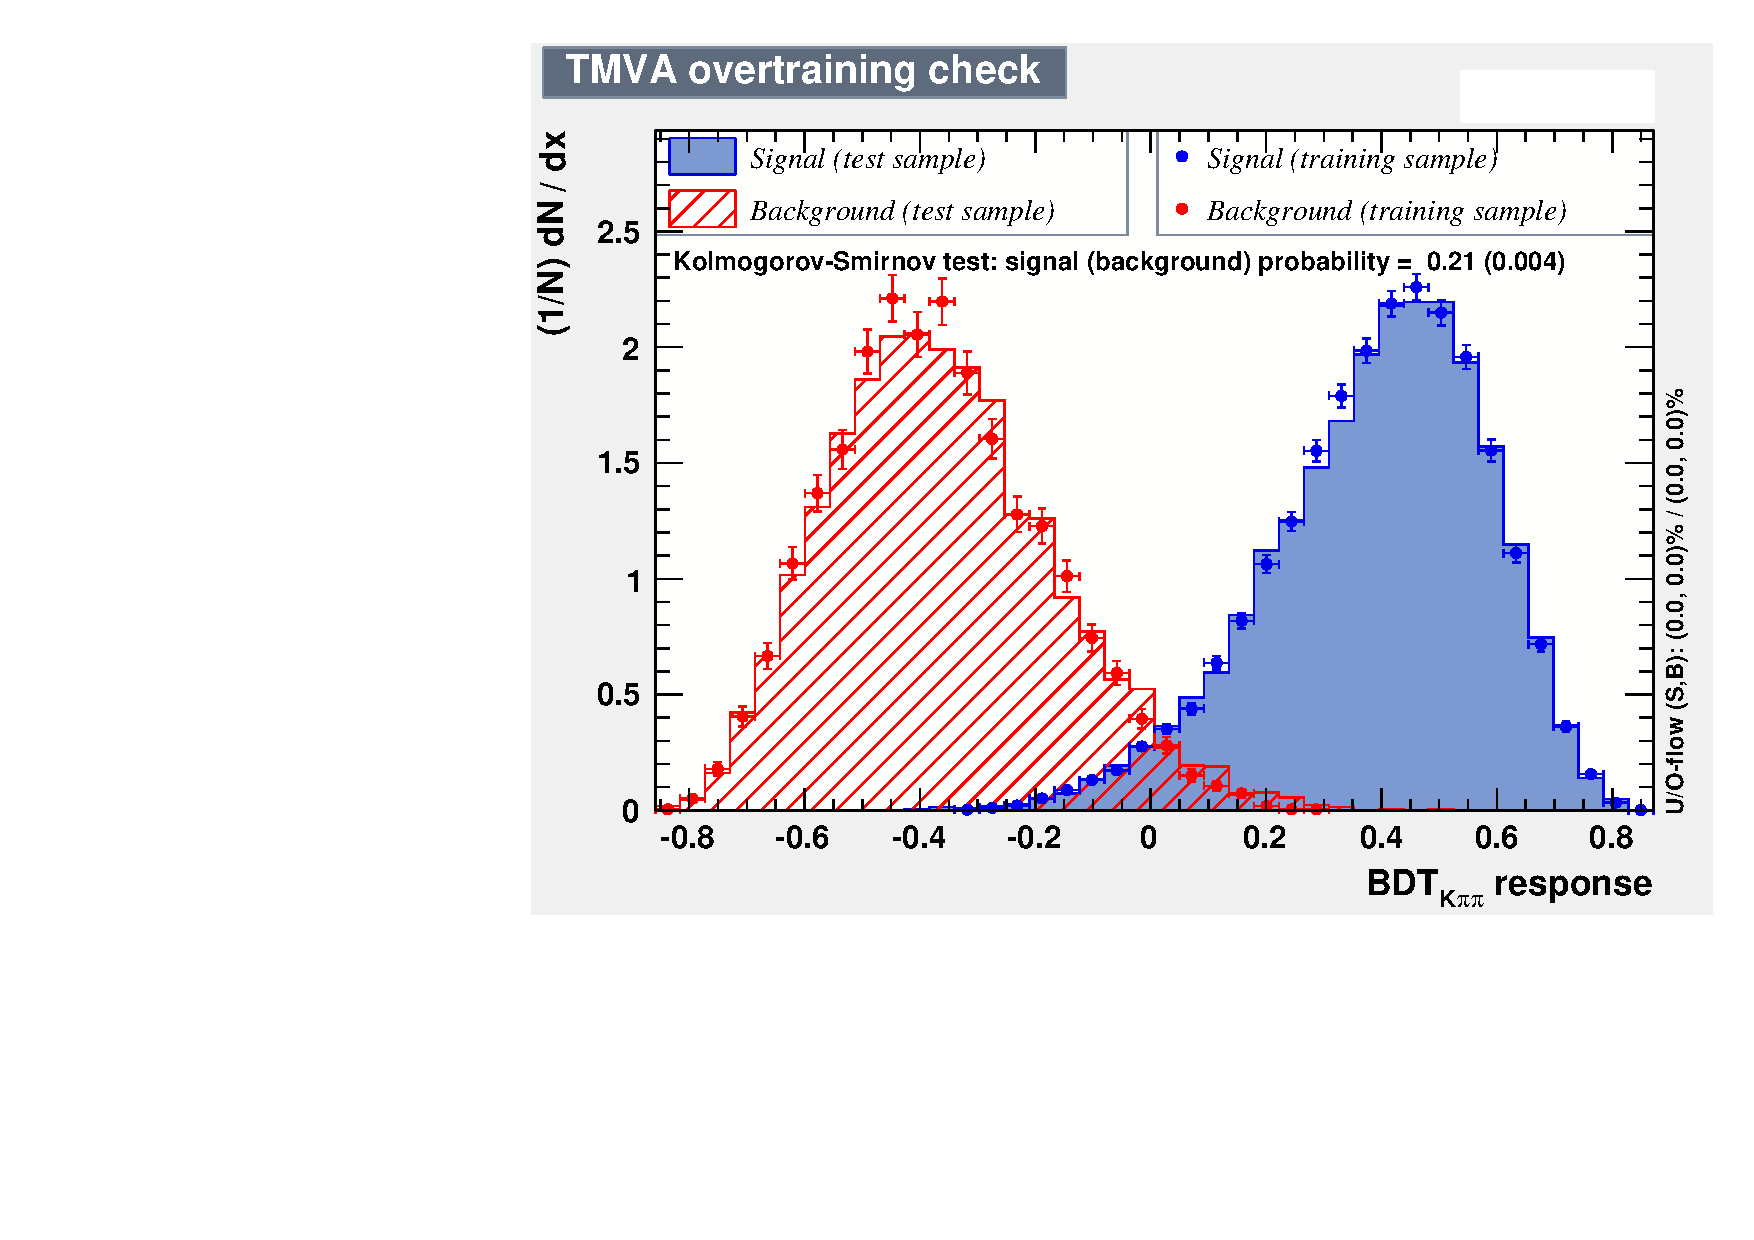
\includegraphics[width=0.48\textwidth]{07-B02DD/figs/Overtraining_Check_Kpipi.pdf}
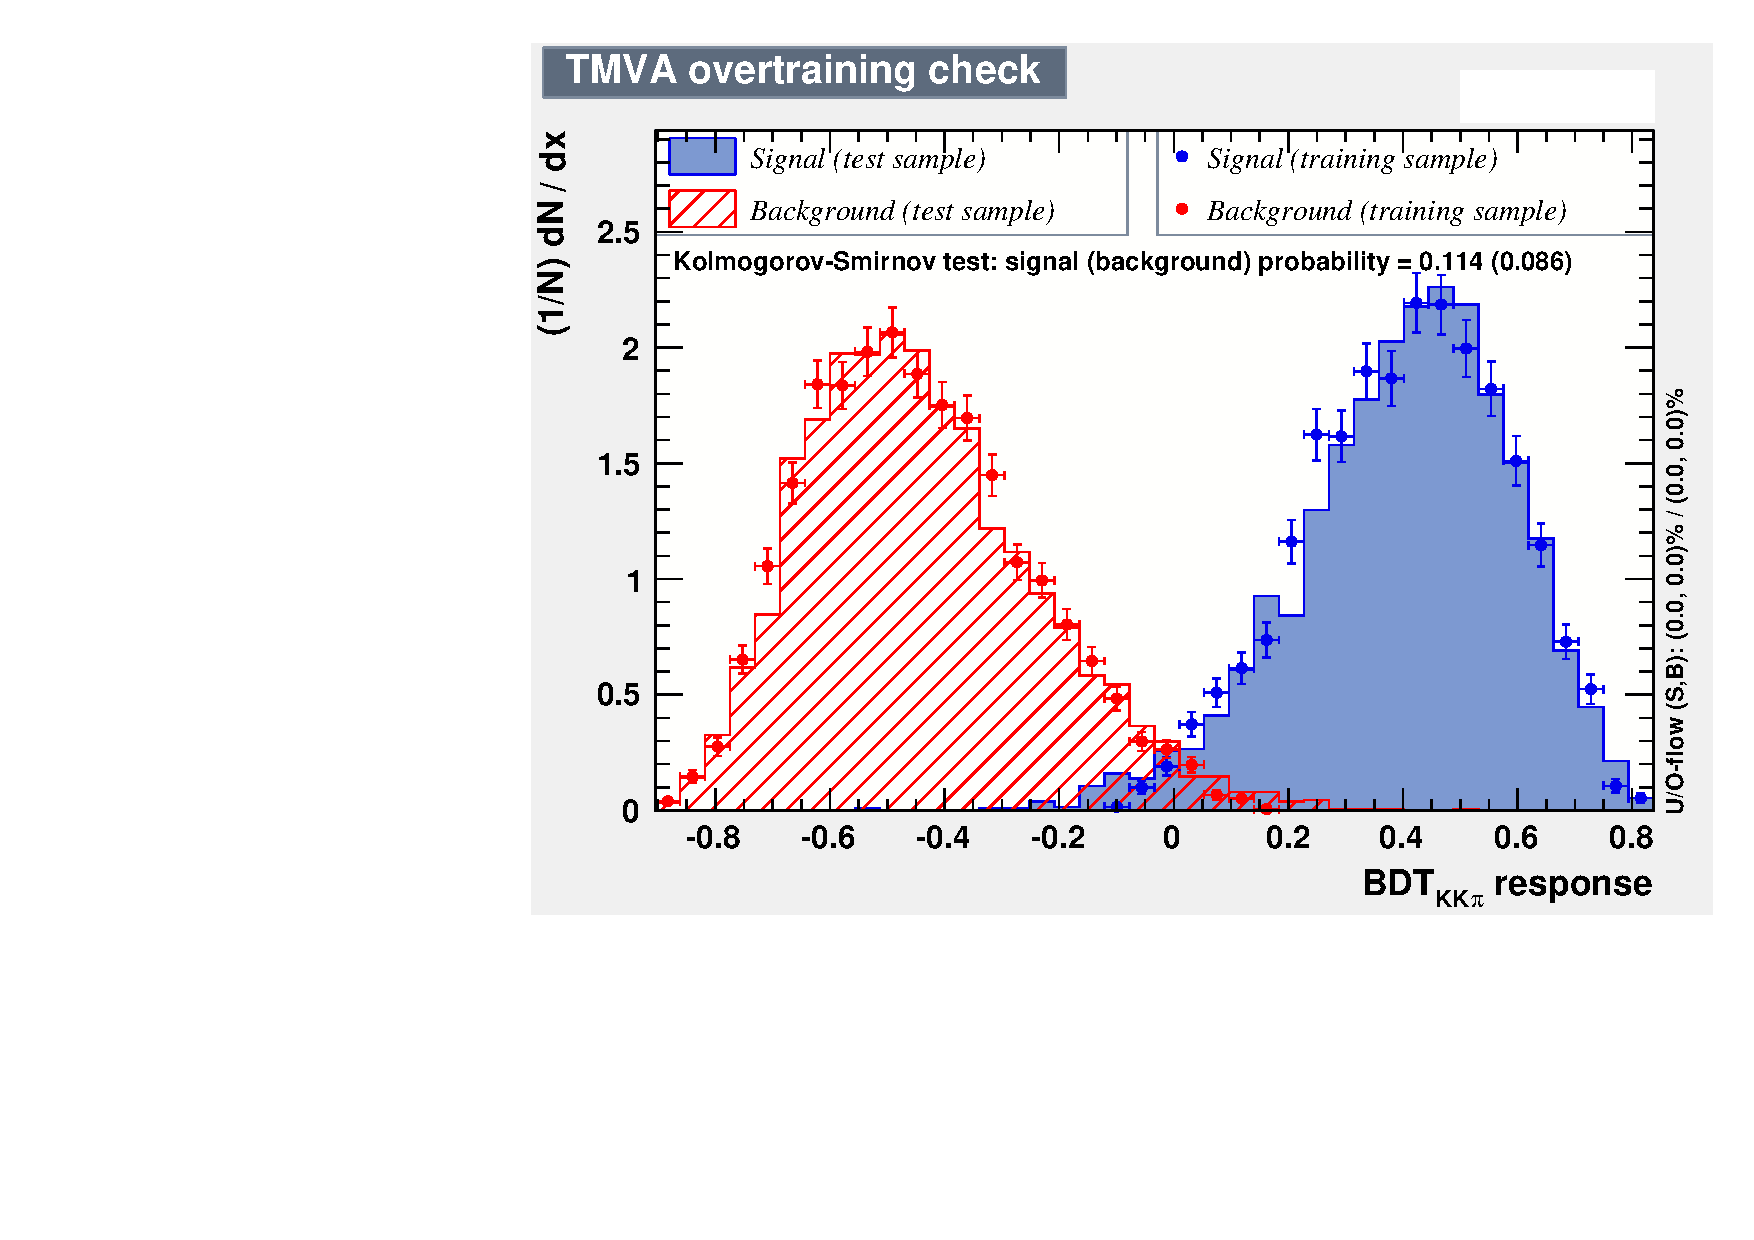
\includegraphics[width=0.48\textwidth]{07-B02DD/figs/Overtraining_Check_KKpi.pdf}
\caption{Comparison of the BDT response on training and test sample for the
\KpipiKpipi final state (left) and the \KKpiKpipi final state (right).}
\label{fig:b02dd:selection:mva:overtraining}
\end{figure}
%
Using simulations in the selection contains the possibility that certain
distributions are not modelled properly and differences between the simulation
and real data are exploited instead of differences between signal and
background. Indeed, the classifier output distributions of the signal MC and
background-subtracted data show a quite large disagreement for both final
states as can be seen in \cref{fig:b02dd:selection:mva:bdtcomparison}. The
performance is clearly overestimated in the training.
%
\begin{figure}[htbp]
    \centering
    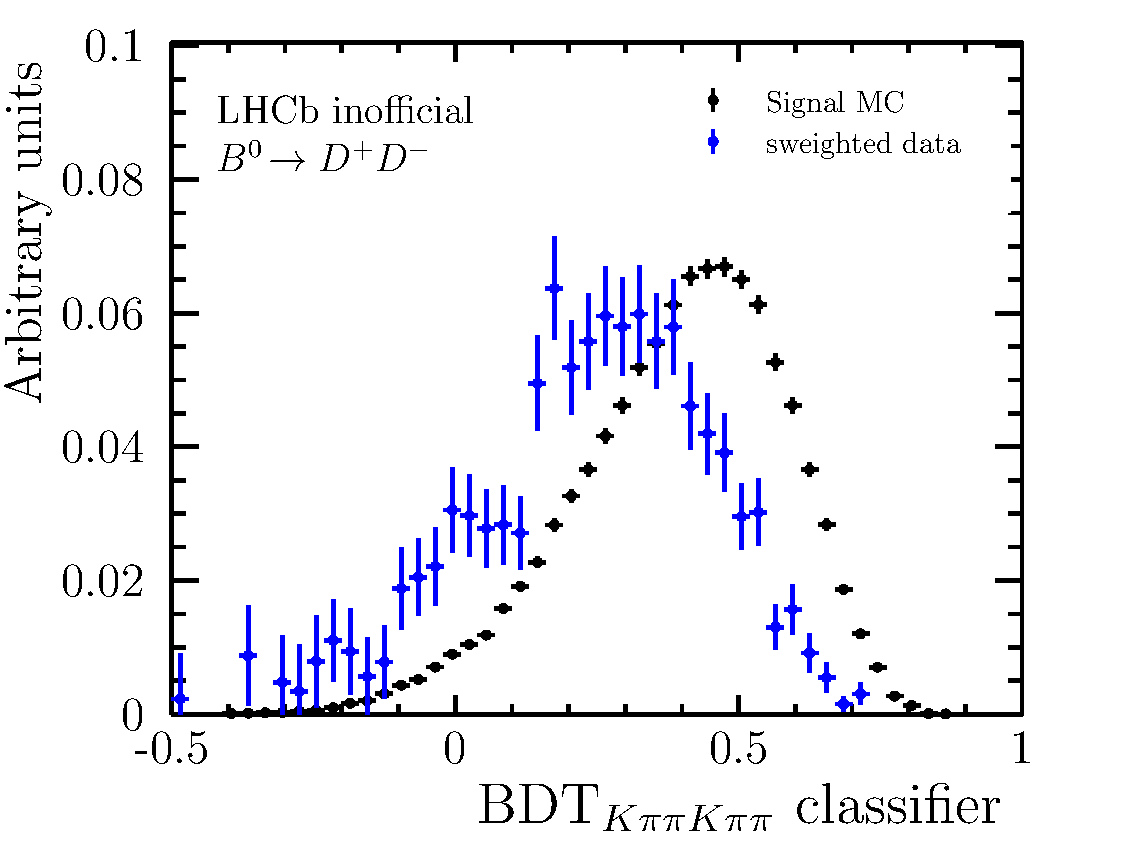
\includegraphics[width=0.49\textwidth]{07-B02DD/tikz/pdf/BDTComparison_Kpipi.pdf}
    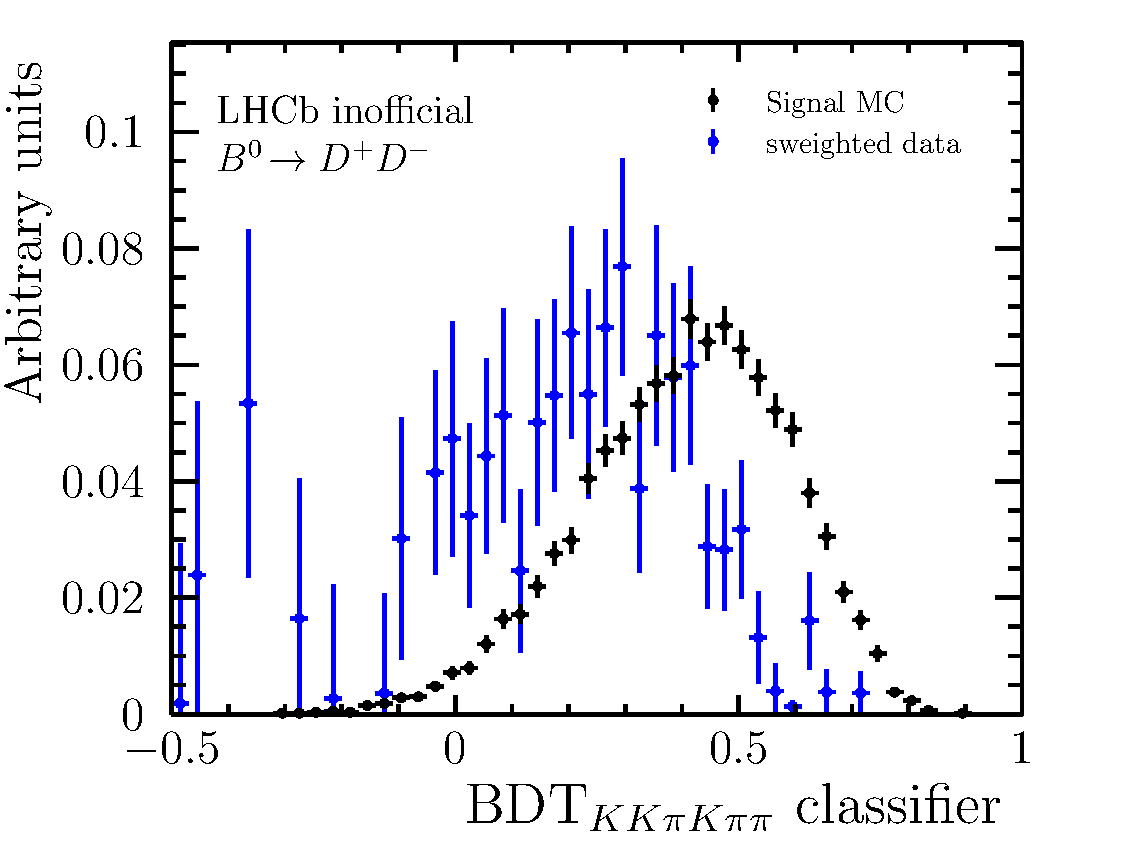
\includegraphics[width=0.49\textwidth]{07-B02DD/tikz/pdf/BDTComparison_KKpi.pdf}
    \caption{Distribution of the BDT output for background-subtracted data (blue) and
    signal MC (black) for the \KpipiKpipi final state (left) and the
    \KKpiKpipi final state (right).}
    \label{fig:b02dd:selection:mva:bdtcomparison}
\end{figure}
%
This would be a problem if the selection efficiencies had to be calculated
using the MC sample. But for a measurement of \CP violation it is mainly
important that the amount of background can somehow be reduced while most of
the signal is kept. This can be achieved with the current setting.

% ==============================================================================
\subsubsection*{BDT cut optimisation}
\label{sec:b02dd:selection:mva:optimisation}

As explained in \cref{sec:dataanalysis:selection:fom} the best figure of merit
for a measurement of \CP violation is the sensitivity on the \CP observables
themselves. So the requirement on the BDT classifier output is scanned
performing a fit to the invariant $\Dp\Dm$ mass spectrum followed by a decay
time fit of the background-subtracted sample for each scan point. Initially,
only the subsample with two kaons in the \Bd final state is analysed. In
\cref{fig:b02dd:selection:mva:sensitivities} the statistical
uncertainties of \SDD and \CDD are plotted as a function of the requirement on
the BDT classifier output.
%
\begin{figure}[!htb]
\centering
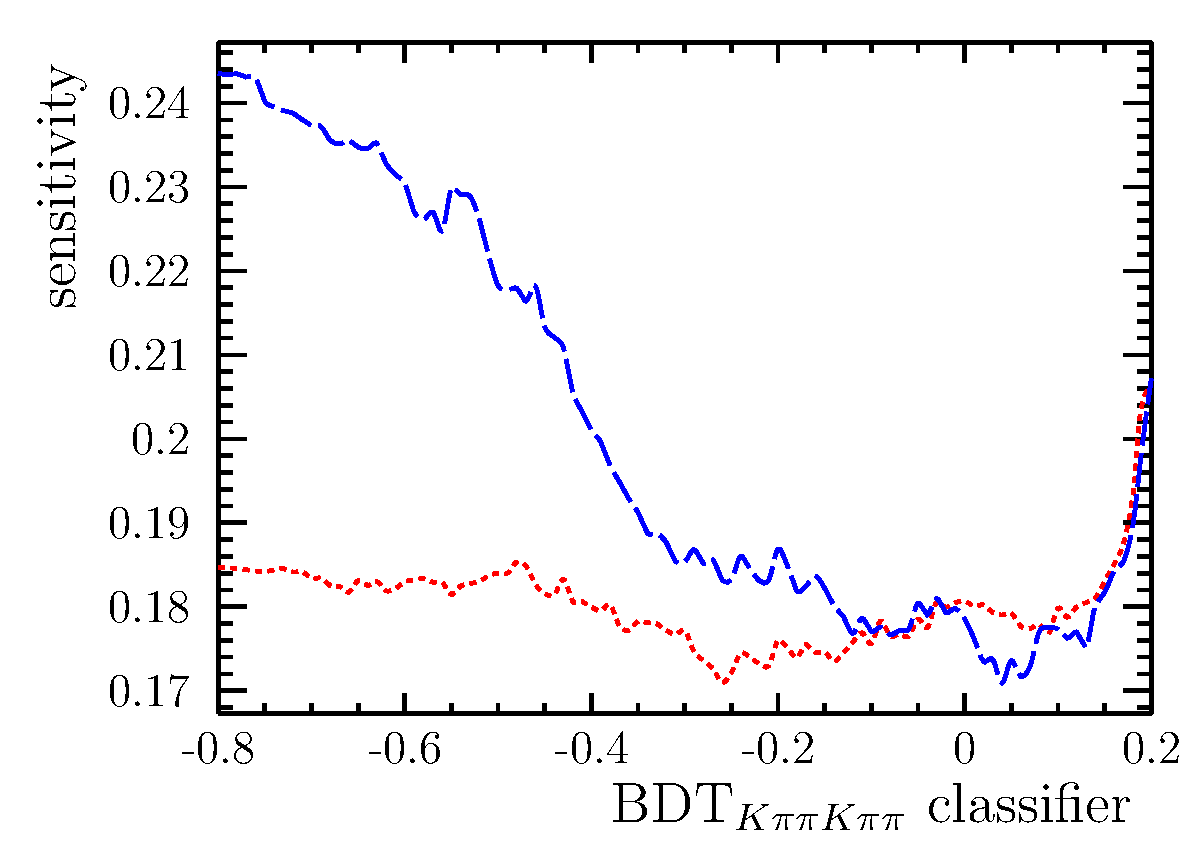
\includegraphics[width=0.48\textwidth]{07-B02DD/tikz/pdf/Sensitivities_Kpipi.pdf}
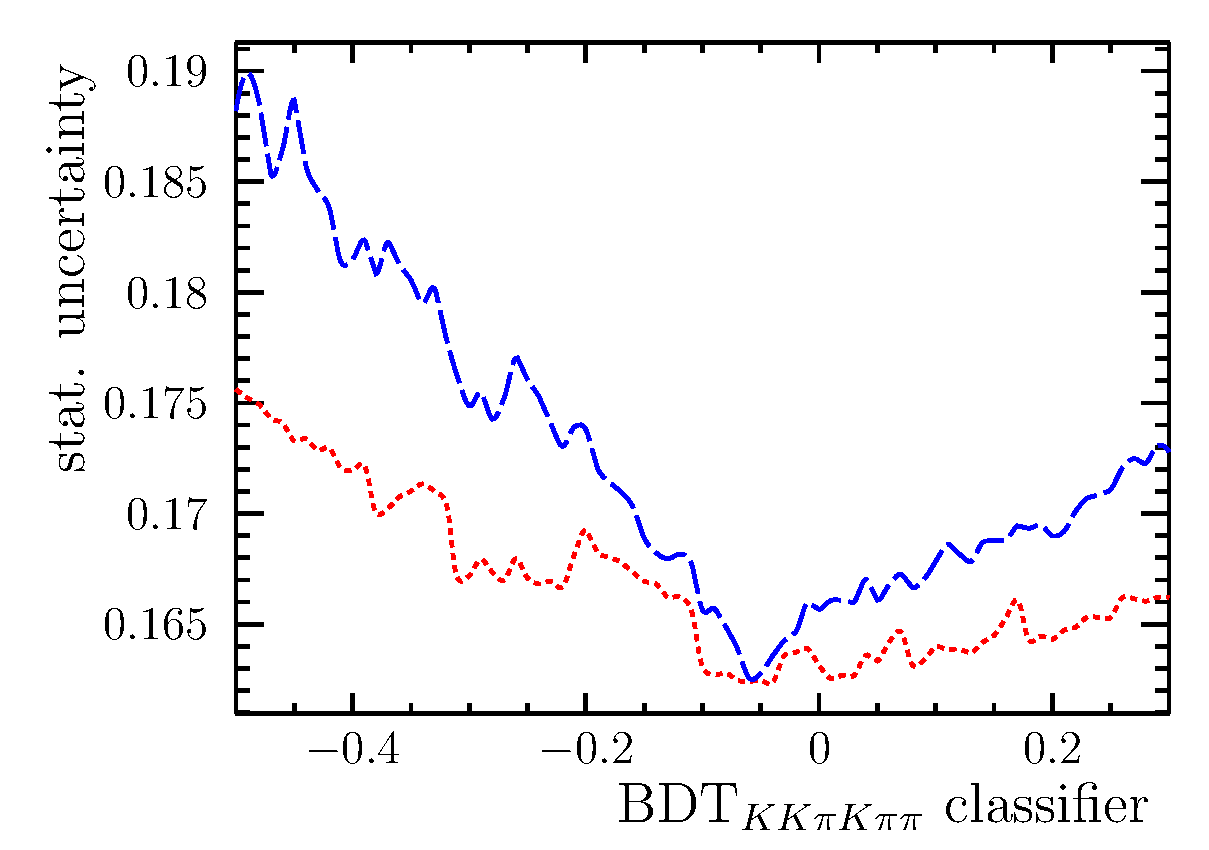
\includegraphics[width=0.48\textwidth]{07-B02DD/tikz/pdf/Sensitivities_KKpi.pdf}
\caption{Sensitivity of \SDD (red short-dashed) and \CDD (blue long-dashed) as
a function of the BDT classifier output for the \KpipiKpipi final state (left)
and the \KKpiKpipi final state (right).}
\label{fig:b02dd:selection:mva:sensitivities}
\end{figure}
%
The uncertainty on \CDD improves with tighter requirements on the BDT
classifier until it reaches an optimum shortly after zero. This can be
explained with the fact that the sensitivity on \CDD mainly comes from
candidates at low decay times because the cosine function is maximal there.
The suppression of the rather short-lived combinatorial background compensates
the loss in signal efficiency for a quite long range. In contrast, the
uncertainty on \SDD is mainly driven by the amount of signal candidates. So it
is more or less flat for loose requirements on the BDT classifier where only
few signal candidates are lost and this is compensated by the higher purity
and reaches its optimum around \num{-0.25} before it starts to get worse. Now
that both observables are of interest and the optima are not at the same cut
value it is decided to require the BDT classifier to be greater than
\num{-0.10}. This is a good compromise between both observables as the
uncertainties of \SDD and \CDD are almost the same and close to their optima.
The requirement has a signal efficiency of \SI{96.5\pm0.5}{\percent} and
rejects \SI{84.18\pm0.34}{\percent} of the combinatorial background.

In a second step the requirement on the BDT classifier for the \KKpiKpipi
final state is optimised. The \KKpiKpipi subsample is quite small, which makes
individual fits on this subsample rather unstable. This can be solved by
performing a simultaneous fit to the whole dataset with the previously
determined BDT cut applied to the \KpipiKpipi subsample. Scanning the BDT
classifier output for the \KKpiKpipi final state results in the sensitivities
on \SDD and \CDD plotted in \cref{fig:b02dd:selection:mva:sensitivities}. Both
uncertainties show a minimum at around \num{-0.05}, which is chosen as cut
value. This cut removes \SI{90.75\pm0.33}{\percent} of the combinatorial
background at a signal efficiency of \SI{87.2\pm1.9}{\percent}.

\subsection{Final selection}
\label{sec:b02dd:selection:final_selection}

Finally, the fit range of the invariant $m_{\Dp\Dm}$ mass is reduced to
\SIrange{5150}{5500}{\MeVcc}, which eliminates some backgrounds, like
misreconstructed \mbox{\BdToDstD}, at low masses, prevents overtraining
effects on the high-mass sideband used in the training of the BDT, and leaves
enough candidates in the upper mass sideband to determine the shape of the
combinatorial background. Additionally, the decay time is restricted to be in
the range \SIrange{0.25}{10.25}{\ps} to avoid edge effects. In
\SI{0.8}{\percent} of the selected events more than one candidate remains,
which is very unlikely given the low branching fraction. Therefore, only one
of the multiple candidates is kept, which is chosen randomly.
